You want to design a PD controller 
\[
C(s) = K_p + K_ds = K_d \left( s + \frac{K_p}{K_d} \right)
\]
to control the angular position of a satellite that is part of NOAA's Search and Rescue Satellite Aided Tracking (SARSAT) system \footnote{\url{http://www.sarsat.noaa.gov/}}. The block diagram for the closed-loop system with reference position $\theta_{ref}$ and actual position $\theta$ is shown below, where
\[
H(s) = \frac{10}{s+10}
\]
is the sensor used to measure the angular position. 

\begin{center}
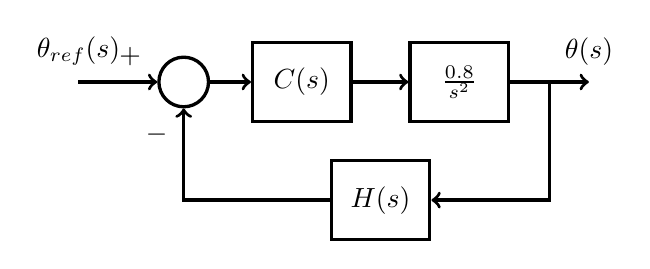
\begin{tikzpicture}[very thick,
sysblock/.style={draw,rectangle,inner sep=6pt,minimum width=1.25cm,minimum height=1.0cm,very thick},
summer/.style={circle,draw,very thick}]

\draw (0,0) node[summer] (sum) {\rule{10pt}{0pt}};
\draw (1.5,0) node[sysblock] (C) {$C(s)$};

\draw (3.5,0) node[sysblock] (G) {$\frac{0.8}{s^2}$};

\draw (2.5,-1.5) node[sysblock] (H) {$H(s)$};

\draw[<-] (sum.180) node[above left=2pt] {$+$} -- ++(-1,0) node[above=2pt] {$\theta_{ref}(s)$};
\draw[->] (sum.0) -- (C.180);
\draw[->] (C.0) -- (G.180);
\draw[->] (G.0) -- ++(0.5,0) |- (H.0);
\draw[->] (H.180)  -| (sum.-90) node[below left=2pt] {$-$};
\draw[->] (G.0) ++(0.5,0) -- ++(0.5,0) node[above=2pt] {$\theta(s)$};

\end{tikzpicture}
\end{center}

To ensure that the SARSAT system can accurately pinpoint and track the location of people in distress, it is required that the closed-loop system controlling the satellite have zero steady-state error to a unit step reference input, a rise time of less than 10 seconds, and a percent overshoot of less than 20\%. Use Bode and Time-Frequency techniques and Matlab (Command Window, \texttt{sisotool}, and/or Simulink) to design the PD controller, verifying that your specifications are met by viewing the step response. Note: you can import the sensor $H(s)$ into \texttt{sisotool} within the \texttt{Control and Estimation Tools Manager} by clicking on \texttt{Architecture-->System Data}.

\begin{enumerate}[(a)]
\item What is the required System Type to meet the steady-state error requirements? Will a PD controller be sufficient?
\item What are the required crossover frequency $\omega_c$ and phase margin $\phi_{PM}$ to achieve the transient specifications?
\item Place the zero at an appropriate location to obtain your desired phase margin.
\item Tune the compensator gain $K_d$ to obtain the desired crossover frequency.
\item Submit a step response plot showing the specifications have been met, a Bode plot showing the phase margin and crossover frequency, and your final values of $K_p$ and $K_d$.
\end{enumerate}

%Please submit your final values of $K_p$ and $K_d$, a step response plot showing that your transient specifications have been met, and a ramp response plot showing that your steady-state error requirement has been met.
